%% ============================================================
%%  Appendix C — Chapter 4 (Comparative) Supporting Information
%%
%%  \include'd from thesis.tex under \appendix, after the
%%  Chapter 2 SI. Holds the methods, provenance, confound-audit,
%%  and per-cell quantitative tables moved out of the main
%%  comparative chapter so its narrative carries only the result.
%% ============================================================

\chapter{Supporting Information for Chapter~\ref*{ch:comparative}}\label{app:ch4_si}

This appendix gathers the analysis provenance, the confound audits, the
fit methodology, and the per-composition-cell quantitative tables that underlie
\cref{ch:comparative}. The main chapter retains the result and the figures; the
material here records how the numbers were produced and lists the per-cell values
behind the heatmaps and design-space plots.

\section{Analysis Provenance and Aggregation}\label{app:ch4_provenance}

\paragraph{Data-quality control.} Two screening layers are applied before any
number is reported, both recorded so that the analysis is reproducible.
Individual measurements that are erratic or non-physical are flagged and
excluded. In addition, a per-device visual review of the recorded curves was
carried out; the resulting verdicts --- whether a curve is used as measured,
cleaned by removing identified anomalous points, or discarded --- together with
the exact points retained, are stored in a curation registry and applied
automatically by the analysis scripts, rather than being made ad hoc. The fitted
timescale obtained directly from the instrument-side pipeline was found not to be
robust to such anomalous points, so all timescales reported in \cref{ch:comparative}
are recomputed after this screening. \Cref{tab:ch4_provenance} records the full
raw-to-summary trail underlying these screened descriptors.

\begin{table}[t]
  \centering
  \caption[Raw-to-summary provenance for the comparative analysis]{Raw-to-summary provenance for the three common measurements used in \cref{ch:comparative}. The same recorded trail underlies the figures of \cref{sec:ch4_composition} and the behavioural models of \cref{ch:temporal}.}
  \label{tab:ch4_provenance}
  \footnotesize
  \setlength{\tabcolsep}{3pt}
  \begin{tabularx}{\linewidth}{@{}>{\raggedright\arraybackslash}p{2.7cm}>{\raggedright\arraybackslash}p{4.5cm}>{\raggedright\arraybackslash}X@{}}
    \toprule
    Stage & Artifact & Role in the analysis \\
    \midrule
    Raw measurement & \path{DEVICES_LAB_DATA/.../D1_all.txt} or split \path{D1_I/V/T.txt} & Keithley current, voltage, and time traces for each device day, measurement type, and crossbar pixel. \\
    Fabrication metadata & \path{DATABASE/UPDATED_DEVICES_LIBRARY.csv} & Canonical device composition, electrode, spin speed, annealing, storage, measurement atmosphere, and operator metadata. \\
    Extracted features & \path{DEVICES_HYST_*}, \path{DEVICES_PULSES_*}, \path{DEVICES_DELAYTIME_*} & Per-curve, per-pixel, and per-device feature tables generated by the archive extraction pipeline. \\
    Exclusion and curation & \path{FILTERED_DEVICES.csv}; \path{handouts/ch4_png_qa_curation.csv} & Red-flag exclusion list plus per-curve visual QA verdicts; retained points are applied by script, not selected separately for each figure. \\
    Recomputed descriptors & \path{handouts/ch4_decay_fits.csv}; \path{handouts/ch4_pulse_descriptors.csv} & Post-curation descriptors: \(t_{1/2}\), identified \(\tau,\beta\) where stable, pulse-growth exponent \(\alpha\), peak ratio, and turnover. \\
    Cell summaries and figures & \path{handouts/ch4_decay_by_cell.csv}; \path{handouts/ch4_pulses_by_cell.csv}; \path{scripts/ch4_comparative_figures.py} & Cell medians, device counts, representative curves, heatmaps, swarm plots, and design-space figures. \\
    \bottomrule
  \end{tabularx}
\end{table}

\begin{table}[p]
  \centering
  \caption[Figure-level provenance for Chapter 4]{Figure-level provenance for the Chapter~4 figures whose detailed file paths are not repeated in the main captions. Script names are relative to the thesis repository; raw measurements reside in the experimental archive paths listed by the scripts.}
  \label{tab:ch4_figure_provenance}
  \scriptsize
  \renewcommand{\arraystretch}{0.92}
  \setlength{\tabcolsep}{2pt}
  \begin{tabularx}{\linewidth}{@{}>{\raggedright\arraybackslash}p{3.1cm}>{\raggedright\arraybackslash}p{4.4cm}>{\raggedright\arraybackslash}X@{}}
    \toprule
    Output & Reproduced by & Principal inputs and audit trail \\
    \midrule
    \Cref{fig:ch4_thickness_control} & \path{scripts/thickness_rpm_audit.py} & \path{DEVICES_PROFILOMETRY_STATS.csv} joined to the screened Chapter~4 descriptors; audit in \path{handouts/14_thickness_rpm_confound_audit.md}. \\
    \Cref{fig:ch4_representative,fig:ch4_composition_heatmaps,fig:ch4_heterogeneity,fig:ch4_potentiation,fig:ch4_design_space} & \path{scripts/ch4_comparative_figures.py} & \path{handouts/ch4_decay_fits.csv}, \path{handouts/ch4_pulse_descriptors.csv}, \path{handouts/ch4_decay_by_cell.csv}, and \path{handouts/ch4_pulses_by_cell.csv}; curve curation in \path{handouts/ch4_png_qa_curation.csv}. \\
    \Cref{fig:ch4_chemistry_landscape,fig:ch4_protocol} & \path{scripts/ch4_comparative_figures.py} & Chemistry-landscape values from the screened descriptor tables; the protocol overlay uses the same-device v114 matched-amplitude comparison recorded in the Chapter~4 audit trail. \\
    \Cref{fig:ch4_iratr} & \path{scripts/ch4_iratr.py}; \path{scripts/ch4_xrd.py} & ATR band extraction in \path{handouts/ch4_iratr_bands.csv}; assessments in \path{handouts/16_iratr_assessment.md} and \path{handouts/17_xrd_assessment.md}. \\
    \Cref{fig:ch4_uvvis} & \path{scripts/ch4_uvvis.py} & 2025 \SY{}/\TMPE{} cation-series UV-Vis spectra; assessment in \path{handouts/18_uvvis_assessment.md}. \\
    \Cref{fig:ch4_eis} & \path{scripts/ch4_eis.py} & \SI{0}{\volt}-DC impedance descriptors from the experimental database, joined to \path{handouts/ch4_decay_by_cell.csv}; per-cell output in \path{handouts/ch4_eis_by_cell.csv}. \\
    \Cref{fig:ch4_electrode} & \path{scripts/ch4_electrode.py} & Silver-versus-gold metrics in \path{handouts/ch4_electrode_by_cell.csv}; audit in \path{handouts/19_electrode_au_assessment.md}. \\
    \bottomrule
  \end{tabularx}
\end{table}

\paragraph{The aggregation ladder.} The aggregation is deliberately
conservative. HYST raw points are first reduced to sweep-level features in
\path{DEVICES_HYST_CURVE_INFO.csv}; broken or FILTERED rows are removed; device
summaries are medians across the surviving sweeps and pixels; and
composition-cell values are medians across devices. PULSES and DELAYTIME follow
the same curve/pixel/device/cell logic, but with protocol-specific descriptors:
the pulse curves are summarised by \(\alpha\), peak ratio, and turnover, while the
decay curves are summarised primarily by \(t_{1/2}\), with \(\tau\) and \(\beta\)
retained only when the fit passes the identification thresholds in
\path{scripts/ch4_dynamics_fits.py}. The representative curves in
\cref{fig:ch4_representative} are selected by the figure script from devices near
the relevant cell medians, so they are illustrative examples of the same
summarized population rather than hand-picked evidence outside the pipeline.

\paragraph{Stretched-exponential identification.} The depotentiation decays are
fitted with the Kohlrausch form of \cref{eq:ch4_kohlrausch}. The
eight-to-thirteen-point decay curves often under-constrain \(\beta\) and \(\tau\)
jointly, so the fitted \(\tau\) is reported only where the fit is well identified,
and the model-free half-enhancement time \(t_{1/2}\) is used as the primary
timescale; where both are available they agree (\cref{tab:ch4_decay_by_cell}).
Fitted \(\beta\) values lie predominantly in \numrange{0.6}{0.9}, i.e. genuinely
stretched relaxation, consistent with the heterogeneous distribution of
activation barriers invoked in \cref{ch:poc}.

\section{Film-Thickness and Fabrication Confound Audits}\label{app:ch4_confounds}

\paragraph{Film thickness is a controlled covariate.} In most batches, the
spin-coating speed was raised for higher-\PEO{} cells to partly equalise
thickness (spanning \SIrange{1500}{3500}{rpm}). The compensation was deliberate
but incomplete: median film thickness still rises from
\(\approx\SI{227}{\nano\meter}\) at \PEO{}~\num{0.3} to
\(\approx\SI{298}{\nano\meter}\) at \PEO{}~\num{1.2}, giving a Pearson
\(r\approx0.68\) between \PEO{} fraction and thickness
(\cref{fig:ch4_thickness_control}).
Four observations show that thickness is nonetheless not the operative variable:
\begin{enumerate}
  \item The reported metrics are dimensionless ratios and timescales (on--off ratio, log--log slope, relaxation time), in which an absolute series-resistance or geometric effect of thickness cancels.
  \item The activation voltage is flat (\SIrange{2.2}{2.4}{\volt}, \(r\approx-0.06\) against thickness) across a \(2.6\times\) thickness range, so the switching threshold is an intrinsic ionic property rather than a bulk-field effect that would scale with film thickness.
  \item Within the single lead cell (\PEO{}~\num{0.3}/salt~\num{0.09}) a \(38\%\) device-to-device thickness spread (\SIrange{196}{271}{\nano\meter}) leaves the fading-memory time essentially unchanged (\(t_{1/2}\approx\SIrange{18}{22}{\second}\)).
  \item Decisively, once composition is held fixed the thickness correlation with \(\log t_{1/2}\) vanishes (partial \(r\approx+0.05\)), while the \PEO{} effect survives after controlling for thickness (partial \(r\approx-0.42\)); the same holds for the potentiation metrics.
\end{enumerate}
Thickness covaries with \PEO{} as a downstream consequence of polymer loading, but
the dynamics track composition. The full join and statistics are reproduced by
\path{scripts/thickness_rpm_audit.py} and
\path{handouts/14_thickness_rpm_confound_audit.md}.

\paragraph{Other fabrication variables are held constant or crossed.} The full
per-device fabrication record was audited to confirm that the composition trends
are not driven by some other processing variable. Across the silver composition
grid the principal process levers are held \emph{constant}: the annealing
temperature (\SI{75}{\celsius}, no second stage), the electrode (\SI{100}{\nano\meter}
silver, evaporated by the same operator), the semiconductor loading, the solvent,
and --- importantly for a hygroscopic polyether --- storage \emph{and} measurement
under a glovebox atmosphere, so ambient humidity is controlled out. The variables
that do change across the grid (fabrication batch and date, the operator who
prepared the solutions, the semiconductor lot, and the device age at measurement)
are \emph{crossed} with composition rather than confounded with it: each
composition cell is populated from several independent batches, and within any
single batch every composition level was fabricated together and measured on the
same day. The composition trends are accordingly reproduced \emph{within}
individual single-day batches --- including one in which the spin speed was held
fixed across all compositions, so that the trend appears with no thickness
compensation at all. The full column-by-column audit is recorded in
\texttt{handouts/15\_fabrication\_confound\_audit.md} and reproduced by
\texttt{scripts/fabrication\_confound\_audit.py}.

\section{Per-Composition-Cell Summaries}\label{app:ch4_celltables}

\Cref{tab:ch4_decay_by_cell,tab:ch4_pulses_by_cell} list the per-cell values
behind the heatmaps of \cref{sec:ch4_composition} and the design space of
\cref{fig:ch4_design_space}. Each row is a composition cell; values are medians
over the screened devices in the cell, with the device count \(n\) given so that
the replicated \ce{Li+} composition spine is distinguished from the
single-device \ce{Na+}/\ce{K+} chemistry points.

\begin{table}[t]
  \centering
  \caption[Per-cell fading-memory descriptors]{Fading-memory (DELAYTIME) descriptors per composition cell, silver electrode, matched \SI{4}{\volt}/\SI{2}{\volt} protocol. \(t_{1/2}\): model-free half-enhancement time (s). \(R_{60}\): retention at \SI{60}{\second}. \(\tau,\beta\): Kohlrausch parameters (median over the \(n_{\mathrm{id}}\) devices with an identified fit). Em-dash: not identified.}
  \label{tab:ch4_decay_by_cell}
  \footnotesize
  \setlength{\tabcolsep}{5pt}
  \begin{tabular}{llrrrrrr}
    \toprule
    Cation & \PEO{}/salt & \(n\) & \(t_{1/2}\,(\mathrm{s})\) & \(R_{60}\) & \(n_{\mathrm{id}}\) & \(\tau\,(\mathrm{s})\) & \(\beta\) \\
    \midrule
    \ce{Li+} & 0.15/0.18 & 1 & 22.4 & 0.27 & 0 & --- & --- \\
    \ce{Li+} & 0.3/0.045 & 4 & 15.8 & 0.20 & 3 & 25.8 & 0.64 \\
    \ce{Li+} & 0.3/0.09  & 3 & 19.2 & 0.28 & 2 & 23.9 & 0.83 \\
    \ce{Li+} & 0.6/0.045 & 3 & 3.3  & 0.06 & 1 & 3.0  & 0.97 \\
    \ce{Li+} & 0.6/0.09  & 3 & 3.5  & 0.02 & 1 & 3.0  & 0.61 \\
    \ce{Li+} & 0.6/0.18  & 2 & 5.5  & 0.04 & 2 & 4.6  & 0.61 \\
    \ce{Li+} & 1.2/0.045 & 3 & 2.7  & 0.13 & 0 & --- & --- \\
    \ce{Li+} & 1.2/0.09  & 3 & 6.0  & 0.09 & 2 & 6.9  & 1.08 \\
    \ce{Li+} & 1.2/0.18  & 3 & 9.0  & 0.13 & 3 & 10.0 & 0.87 \\
    \midrule
    \ce{Na+} & 0.3/0.09  & 1 & 24.0 & 0.42 & 0 & --- & --- \\
    \ce{K+}  & 0.3/0.09  & 1 & 8.0  & 0.22 & 0 & --- & --- \\
    \bottomrule
  \end{tabular}
\end{table}

\begin{table}[t]
  \centering
  \caption[Per-cell potentiation descriptors]{Potentiation (PULSES) descriptors per composition cell, silver electrode, \SI{3}{\volt}/\SI{1.5}{\volt} protocol. \(\alpha\): log--log growth exponent. Peak: peak conductance ratio (\(\times\)). \(N_{\mathrm{peak}}\): pulse count at peak. Turnover: fraction of devices whose response turns over within \(N\le\num{1000}\).}
  \label{tab:ch4_pulses_by_cell}
  \footnotesize
  \setlength{\tabcolsep}{5pt}
  \begin{tabular}{llrrrrr}
    \toprule
    Cation & \PEO{}/salt & \(n\) & \(\alpha\) & Peak (\(\times\)) & \(N_{\mathrm{peak}}\) & Turnover \\
    \midrule
    \ce{Li+} & 0.15/0.045 & 1 & 0.06 & 1.4   & 100  & 100\% \\
    \ce{Li+} & 0.3/0.045  & 4 & 1.11 & 482.6 & 300  & 100\% \\
    \ce{Li+} & 0.3/0.09   & 4 & 0.90 & 149.9 & 1000 & 0\% \\
    \ce{Li+} & 0.3/0.18   & 2 & 0.18 & 3.8   & 1000 & 0\% \\
    \ce{Li+} & 0.6/0.045  & 3 & 0.57 & 14.8  & 100  & 100\% \\
    \ce{Li+} & 0.6/0.09   & 3 & 0.83 & 202.3 & 300  & 100\% \\
    \ce{Li+} & 0.6/0.18   & 3 & 0.63 & 76.9  & 1000 & 0\% \\
    \ce{Li+} & 1.2/0.045  & 3 & 0.33 & 4.4   & 100  & 100\% \\
    \ce{Li+} & 1.2/0.09   & 2 & 0.49 & 42.6  & 1000 & 0\% \\
    \ce{Li+} & 1.2/0.18   & 3 & 0.37 & 8.0   & 1000 & 0\% \\
    \midrule
    \ce{Na+} & 0.3/0.09   & 1 & 0.27 & 10.0  & 1000 & 0\% \\
    \ce{K+}  & 0.3/0.09   & 1 & 0.86 & 103.2 & 300  & 100\% \\
    \bottomrule
  \end{tabular}
\end{table}

\section{Realised Device Palette}\label{app:ch4_palette}

The quantitative analyses of \cref{ch:comparative} are deliberately confined to
the replicated silver \PEO{}/\LiTf{} composition spine. It is nonetheless useful
to see the full set of behaviours the device family actually realises, because it
is this realised spread --- not any single optimised cell --- that the temporal
chapter treats as a computational resource. \Cref{fig:ch4_palette} places every
silver device that carries both a measured switching window and a measured fading
timescale (\(n=54\), all hosts, cations and anions; FILTERED-flagged and broken
pixels removed; device medians) in a single window-versus-retention map. The map
is descriptive only: the chemistry axes are illustrative (\cref{sec:ch4_chemistry})
and no comparative claim is drawn from it. Two features are worth noting. The
populated region spans more than an order of magnitude in both axes, so the
substrate offers a broad palette of \((\text{window},\tau)\) operating points.
And the lead composition is not an isolated point but a cluster of replicate
devices spread over \(\tau\approx\SIrange{0.4}{20}{\second}\), the visual
counterpart of the within-cell device-to-device scatter quantified in
\cref{app:ch5_scatter}.

\begin{figure}[t]
  \centering
  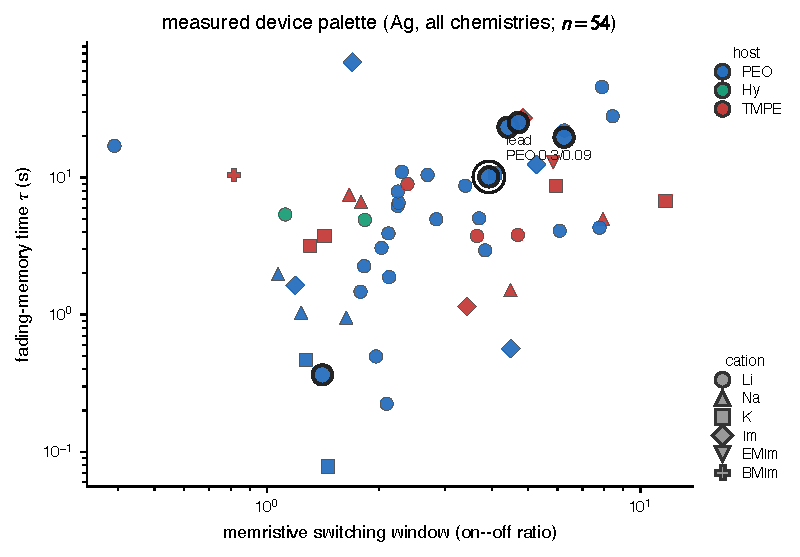
\includegraphics[width=0.82\linewidth]{../figures/chapter4/palette.pdf}
  \caption[Realised device palette across the library]{Measured window-versus-retention palette of the silver device library (\(n=54\) devices with both a clean hysteresis window and a fading-memory fit, all chemistries). Colour encodes the ion-conductor host, marker encodes the salt cation; the lead \PEO{}~0.3/0.09 cell is ringed. The cloud spans over a decade in each axis, and the lead-cell replicates alone span \(\tau\approx\SIrange{0.4}{20}{\second}\). Descriptive overview only; the quantitative claims of \cref{ch:comparative} rest on the replicated composition spine, not on this map.}
  \label{fig:ch4_palette}
\end{figure}

\section{Impedance: Equivalent Circuit and Per-Cell Values}\label{app:ch4_eis_detail}

\paragraph{Equivalent-circuit model.} Beyond the model-free Nyquist-apex
resistance used in \cref{sec:ch4_eis}, each spectrum was also summarised by the
bulk ionic resistance \(R_{\mathrm{ion}}\) of an equivalent circuit adapted from
the polymer light-emitting electrochemical cell analysis of Munar \textit{et
al.}~\cite{Munar2012}, in which a series cable term is placed in parallel with
(i) the semiconductor electronic branch (effectively open at \SI{0}{\volt}),
(ii) a geometric constant-phase element, and (iii) an ionic branch of two
interfacial double layers in series with \(R_{\mathrm{ion}}\). Two cautions
apply. First, the archive holds two automated fits of this circuit; the
freely-fitted one (with per-parameter error estimates) tracks composition
appreciably better than a more tightly bounded variant, and only the former is
used. Second, per-spectrum circuit fits are genuinely ill-conditioned --- an
independent refit confirms that several do not converge robustly --- so
\(R_{\mathrm{ion}}\) is reported only as corroboration of the model-free quantity,
never as a precise number. Both observables nonetheless fall steeply and
monotonically with \PEO{} fraction (\cref{tab:ch4_eis_by_cell}): the model-free
\(Z_{\mathrm{real}}^{\mathrm{apex}}\) at rank correlation \(-0.83\) against \PEO{}
on cell medians, the fitted \(R_{\mathrm{ion}}\) at \(-0.84\).

\begin{table}[t]
  \centering
  \caption[Per-cell impedance summaries]{Equilibrium (\SI{0}{\volt}-DC) impedance per composition cell, silver \SY{}/\PEO{}/\LiTf{}. \(Z_{\mathrm{real}}^{\mathrm{apex}}\): model-free real impedance at the Nyquist apex. \(R_{\mathrm{ion}}\): freely-fitted bulk ionic resistance (corroborative only). \(t_{1/2}\): independently measured fading-memory time, repeated from \cref{tab:ch4_decay_by_cell} for the co-decline of \cref{fig:ch4_eis}b. Em-dash: no matched decay.}
  \label{tab:ch4_eis_by_cell}
  \footnotesize
  \setlength{\tabcolsep}{6pt}
  \begin{tabular}{llrrr}
    \toprule
    \PEO{} & salt & \(Z_{\mathrm{real}}^{\mathrm{apex}}\,(\Omega)\) & \(R_{\mathrm{ion}}\,(\Omega)\) & \(t_{1/2}\,(\mathrm{s})\) \\
    \midrule
    0.15 & 0.045 & \num{2.5e8} & \num{2.3e7} & --- \\
    0.15 & 0.09  & \num{1.7e8} & \num{8.7e6} & --- \\
    0.15 & 0.18  & \num{1.0e8} & \num{8.4e6} & 22.4 \\
    0.3  & 0.045 & \num{5.3e7} & \num{4.0e5} & 15.8 \\
    0.3  & 0.09  & \num{1.3e8} & \num{1.0e6} & 19.2 \\
    0.3  & 0.18  & \num{9.9e7} & \num{4.9e5} & --- \\
    0.6  & 0.045 & \num{5.3e6} & \num{1.4e5} & 3.3 \\
    0.6  & 0.09  & \num{2.6e7} & \num{4.6e4} & 3.5 \\
    0.6  & 0.18  & \num{1.9e7} & \num{8.9e4} & 5.5 \\
    1.2  & 0.045 & \num{4.1e5} & \num{1.9e2} & 2.7 \\
    1.2  & 0.09  & \num{5.6e5} & \num{1.1e4} & 6.0 \\
    1.2  & 0.18  & \num{3.8e7} & \num{1.5e5} & 9.0 \\
    \bottomrule
  \end{tabular}
\end{table}

\section{Electrode-Contrast Per-Cell Values}\label{app:ch4_electrode_table}

\Cref{tab:ch4_electrode_by_cell} lists the per-cell behavioural metrics behind the
silver-versus-gold contrast of \cref{sec:ch4_electrode}, including the host-free
and salt-free negative controls that confirm both the ion-transport polymer and
the dissolved salt are required for the memristive response.

\begin{table}[t]
  \centering
  \caption[Electrode-contrast per-cell metrics]{Per-cell behavioural metrics by top electrode (active silver vs inert gold), at the lead composition \num{0.3}/\num{0.09}. On--off and normalised loop area from HYST; \(V_{\mathrm{act}}\) activation voltage (V); peak ratio and \(\alpha\) from PULSES; \(t_{1/2}\) from DELAYTIME (s). Em-dash: no clean decay/fit at that cell. ``none'' rows are host-free or salt-free negative controls.}
  \label{tab:ch4_electrode_by_cell}
  \footnotesize
  \setlength{\tabcolsep}{4pt}
  \begin{tabular}{llrrrrrr}
    \toprule
    Chemistry & Elec. & on--off & area & \(V_{\mathrm{act}}\) & peak & \(\alpha\) & \(t_{1/2}\) \\
    \midrule
    PEO/Li/OTf  & Ag & 3.25 & 0.33 & 2.38 & 123.5 & 0.89 & 19.2 \\
    PEO/Li/OTf  & Au & 2.00 & 0.12 & 2.74 & 29.4  & 0.45 & 87.2 \\
    TMPE/Li/OTf & Ag & 3.82 & 0.32 & 4.18 & 53.7  & 0.33 & 3.7 \\
    TMPE/Li/OTf & Au & 1.29 & 0.07 & 3.61 & 1.9   & 0.17 & --- \\
    TMPE/Na/OTf & Ag & 5.54 & 0.30 & 3.26 & 497.9 & 1.23 & 3.9 \\
    TMPE/Na/OTf & Au & 1.47 & 0.11 & 6.39 & ---   & ---  & --- \\
    TMPE/K/OTf  & Ag & 7.01 & 0.41 & 3.10 & 237.5 & 1.19 & 5.2 \\
    TMPE/K/OTf  & Au & 1.43 & 0.06 & 5.86 & ---   & ---  & --- \\
    TMPE/Na/TFSI& Ag & 1.76 & 0.10 & 2.38 & 25.1  & 0.46 & --- \\
    Hy/Li/OTf   & Ag & 1.41 & 0.06 & 1.61 & 25.2  & 0.39 & --- \\
    none/Li/OTf & Ag & 0.99 & 0.00 & 1.07 & ---   & ---  & --- \\
    TMPE/none   & Ag & 2.95 & 0.20 & 3.18 & 73.0  & 0.96 & --- \\
    none/none   & Au & 1.03 & 0.01 & 1.29 & 2.8   & ---  & --- \\
    \bottomrule
  \end{tabular}
\end{table}
